\begin{sloppypar}In \sbsref{sbs:callbacks} we explained the modifications made to \ac{DIP} and how a simple variable branch would be implemented.
The \ac{DIP} function \lstinline{chooseBranchSet} calls Dippy's \lstinline{branch_method} at fractional nodes.
The function \lstinline{branch_method} has two inputs supplied by \ac{DIP}:
\begin{enumerate}
\item \lstinline{prob} -- the \lstinline{DipProblem} being solved;
\item \lstinline{sol} -- an indexable object representing the solution at the current node.
\end{enumerate}
We define \lstinline{branch_method} using these inputs and the same PuLP structures used to defined the model, allowing Dippy to access the variables from the original formulation and eliminating any need for complicated indexing.\end{sloppypar}

We can explore custom branching rules that leverage constraints to reduce the symmetry in the solution space of the bin packing problem.
Inefficiencies arise from solvers considering multiple equivalent solutions that have identical objective function values and differ only in the subset of the identical bins used.
One way to address this is to add a constraint that determines the order in which the bins can be considered:
\[ y_i \geq y_{i+1}, i = 1, \ldots, m-1 \]
\lstinputlisting[firstnumber=61,linerange=61-62]{../../examples/Dippy/bpp/bin_pack_func.py}
This change results in a smaller branch-and-bound tree (see figure \ref{fig:bpp_tree2}) that provides the same solution but with bin 0 used in place of bin 3, i.e., a symmetric solution, but with the bins now used ``in order''.
\begin{figure}[htp]
\begin{center}
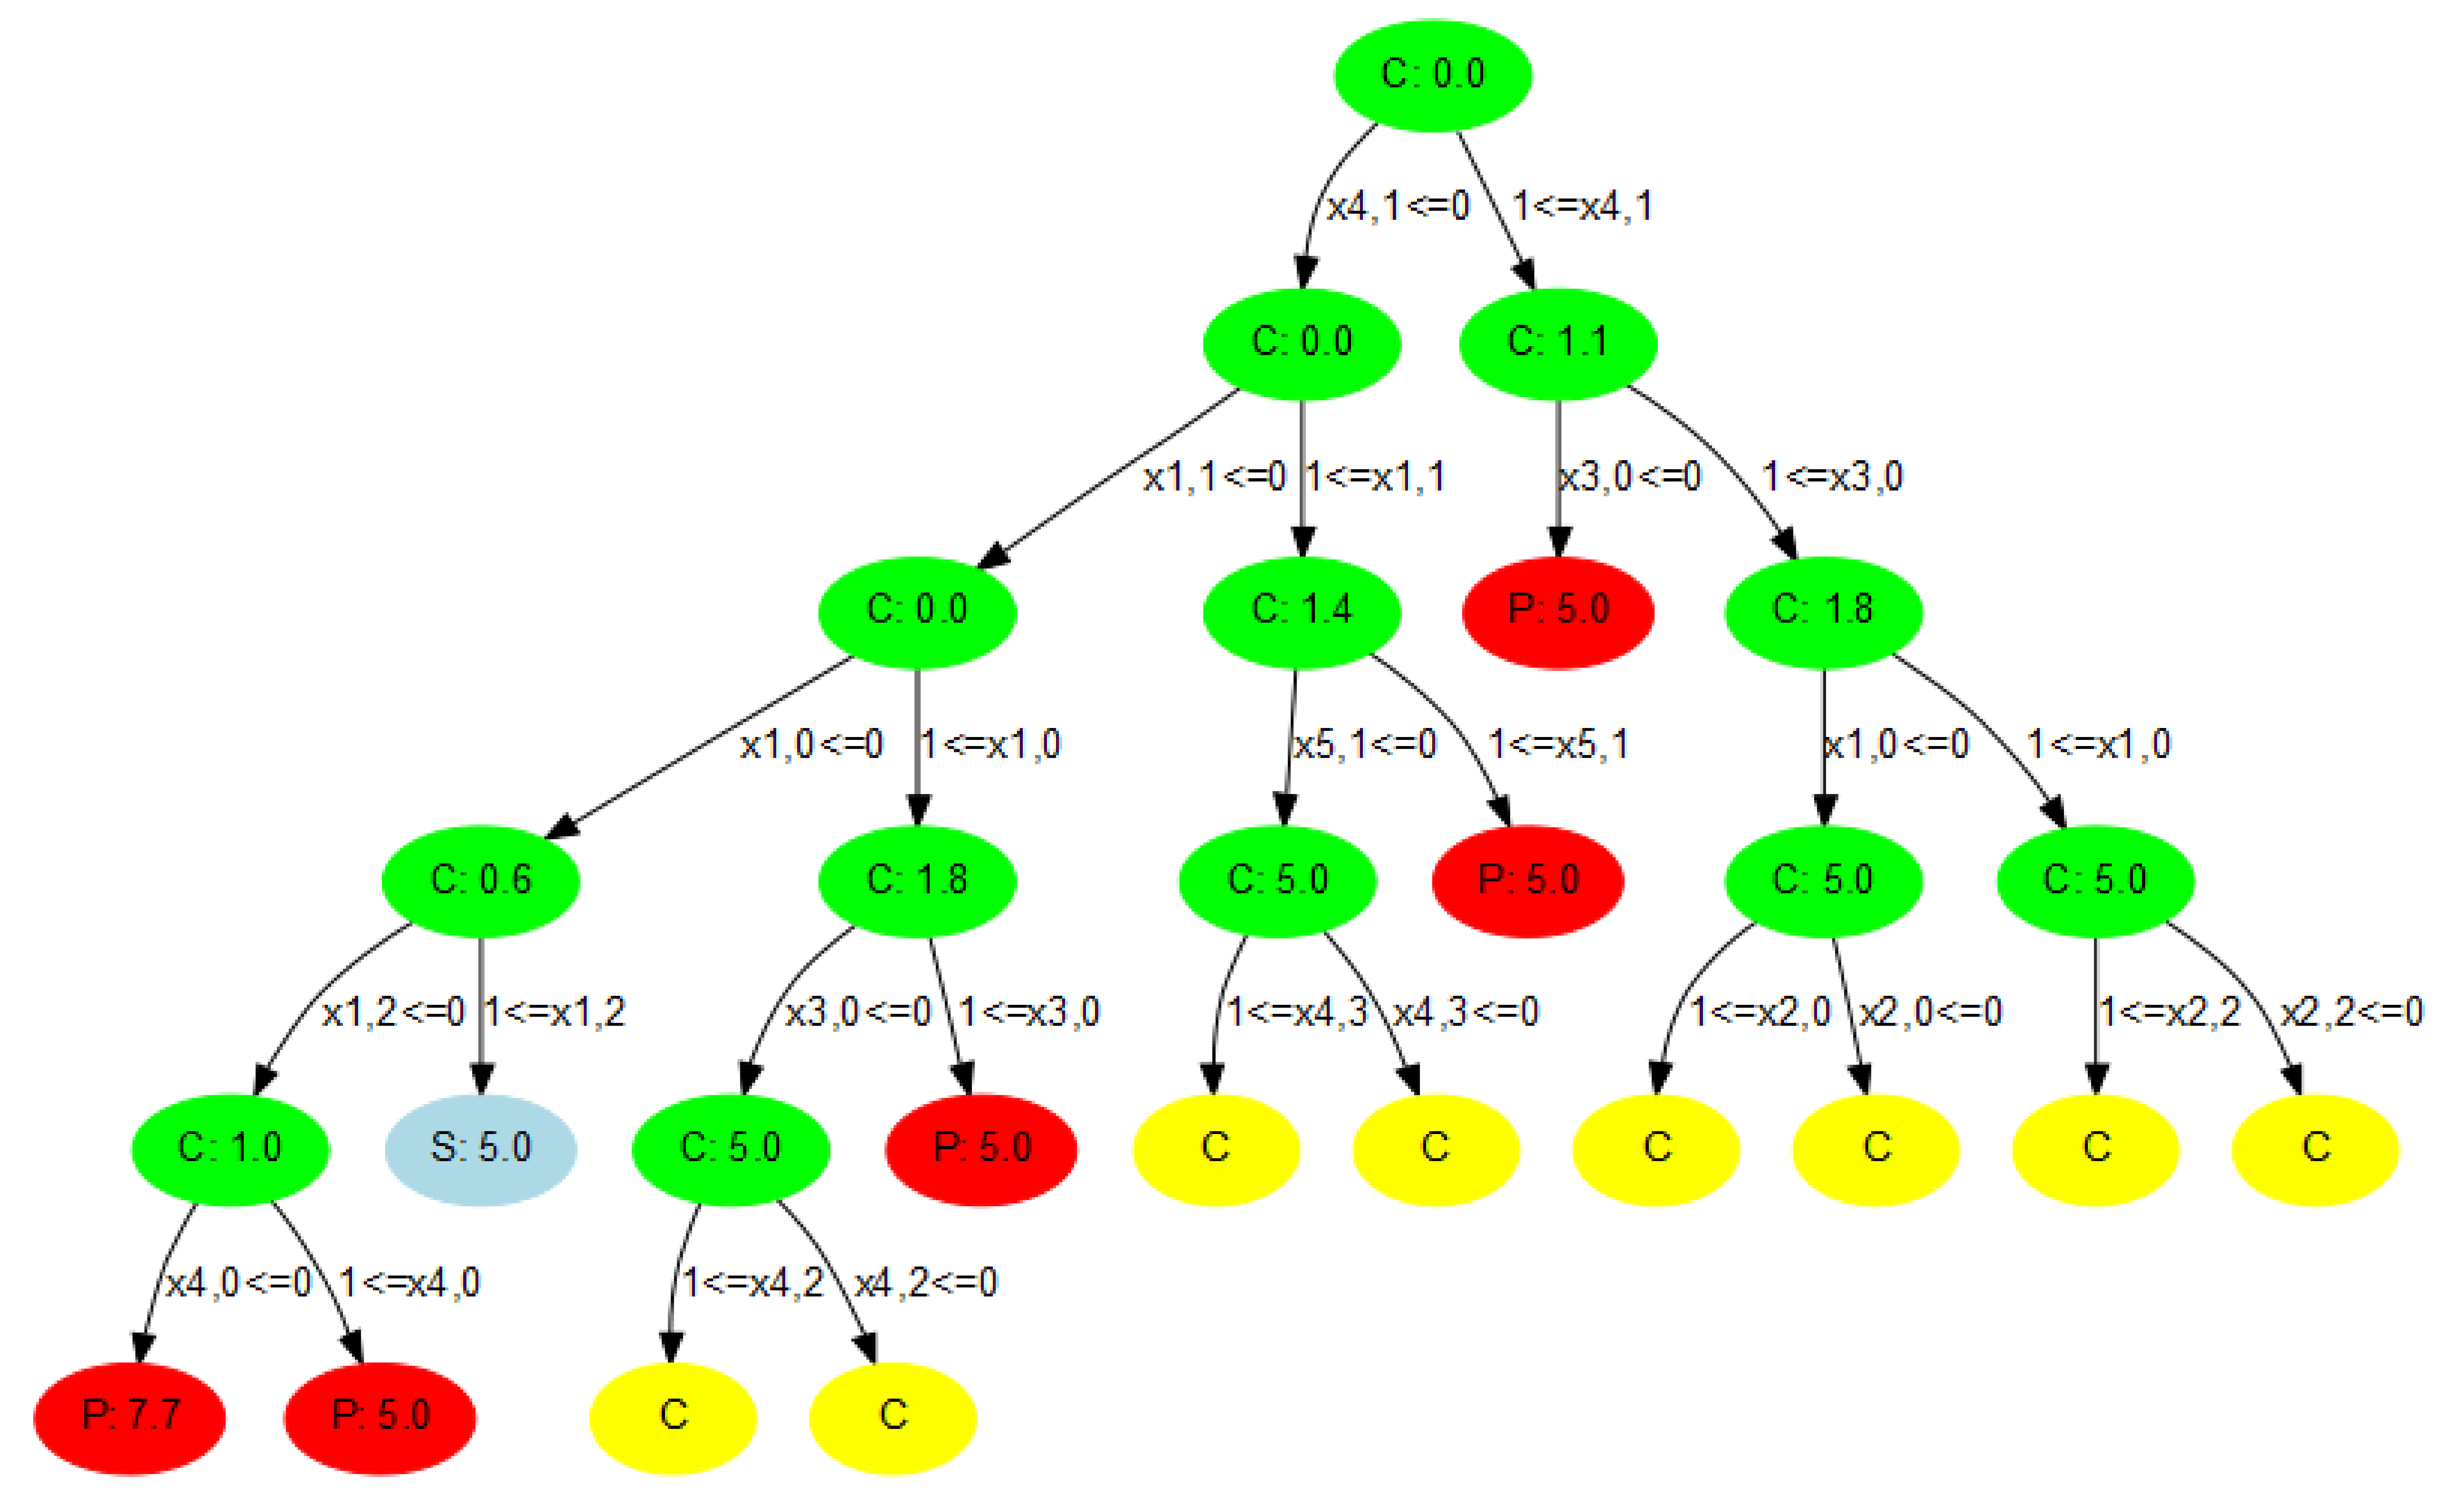
\includegraphics[scale=0.11]{img/bpp_tree2.eps}
\end{center}
\caption{Branch-and-bound tree for bin packing problem instance with anti-symmetry constraints.} \label{fig:bpp_tree2}
\end{figure}

These ordering constraints also introduce the opportunity to implement an effective branch on the number of facilities:

If $\displaystyle\sum_{i=1}^m y_i = \alpha \notin \mathbb{Z}$, then:
\vspace*{-6pt}
\begin{center}
\begin{tabular}{l|l}
the branch down restricts & the branch up restricts \\
$\displaystyle\sum_{i=1}^m y_i \leq \lfloor \alpha \rfloor$ &
$\displaystyle\sum_{i=1}^m y_i \geq \lceil \alpha \rceil$ \\
and the ordering means that & and the ordering means that \\
$y_i = 0, i = \lceil \alpha \rceil, \ldots, m$ &
$y_i = 1, i = 1, \ldots, \lceil \alpha \rceil$
\end{tabular}
\end{center}

\begin{sloppypar}We can implement this branch in Dippy by writing a definition for the \lstinline{branch_method}.\end{sloppypar}
\lstinputlisting[firstnumber=73,linerange={73-75,82-83}]{../../examples/Dippy/bpp/bin_pack_func.py}
\lstinputlisting[firstnumber=182,linerange={182-188,190-193,195-201,203-204,206-207}]{../../examples/Dippy/bpp/bin_pack_func.py}

The advanced branching decreases the size of the branch-and-bound tree further (see figure \ref{fig:bpp_tree3}) and provides another symmetric solution with the bins used in order.
\begin{figure}[htp]
\begin{center}
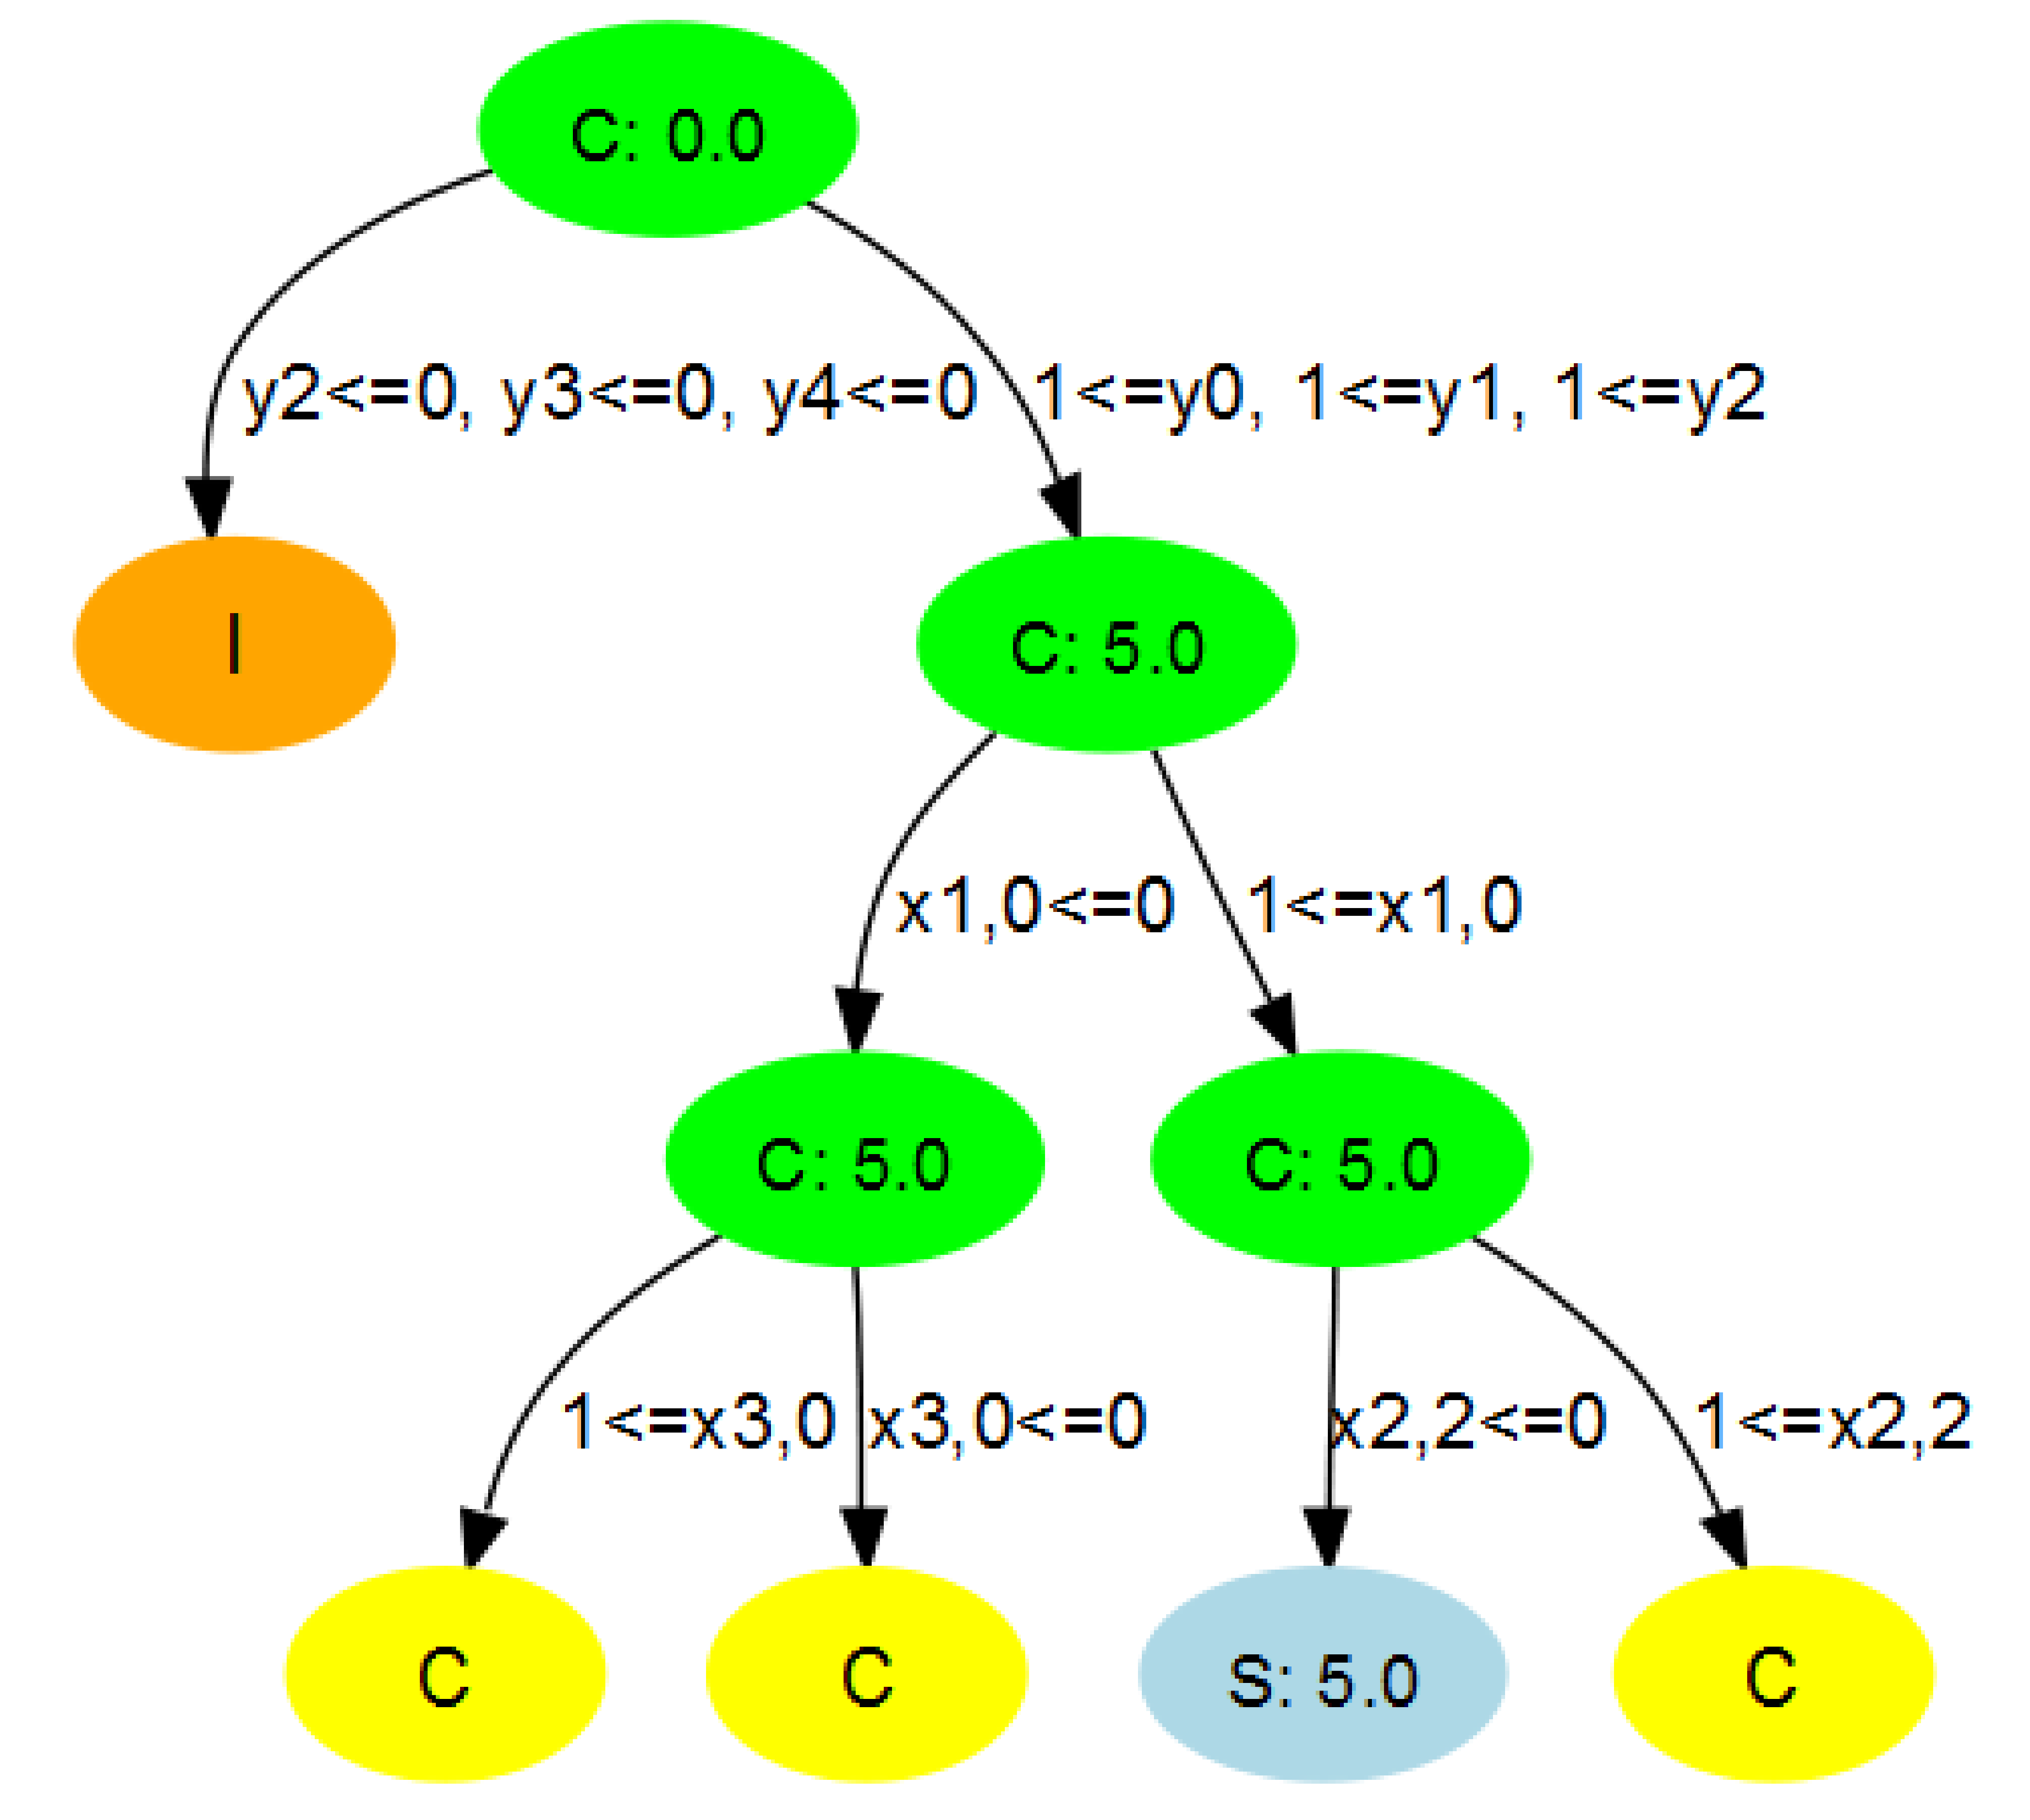
\includegraphics[scale=0.08]{img/bpp_tree3.eps}
\end{center}
\caption{Branch-and-bound tree for bin packing problem instance with anti-symmetry constraints and advanced branching.} \label{fig:bpp_tree3}
\end{figure}
